\section{Declarative Conformance Checking}\label{sec:dccap}
Given that Declare semantics can be expressed as LTL$_f$, we can directly analyse such language having the following syntax:
\[\varphi::=\phi\;|\;\neg \varphi\;|\;\varphi_1\wedge\varphi_2\;|\;\Next \varphi_1\;|\;\varphi_1\Until\varphi_2\]
where $\phi\in \mathsf{Prop}$, while $\Next$ and $\Until$ are respectively the \textit{next} and \textit{until} operators. This is the functionally complete set of connectives, with which we can express  disjunction ($\vee$),  logical implication ($\Rightarrow$),  equivalence ($\Leftrightarrow$), globally ($\Globally$), finally ($\Finally$), weak until ($\Wntil$), and release ($\Release$) as in \cite{XuLZ17a}. Given a finite trace $\sigma=\sigma_1\cdots \sigma_n$ of length $|\sigma|=n$, the satisfiability of $\varphi$ over the $i$-the event in $1\leq i\leq |\sigma|$, namely $\sigma_i\vDash \varphi$, is inductively defined as follows:
\begin{itemize}
	\item $\sigma_i\vDash\phi$ iff. $\sigma_i\vDash\phi$, $\phi\in \mathsf{Prop}$
	\item $\sigma_i\vDash\neg\varphi$ iff. $\sigma_i\not\vDash\varphi$
	\item $\sigma_i\vDash\varphi_1\wedge\varphi_2$ iff. jointly $\sigma_i\vDash\varphi_1$ and $\sigma_i\vDash\varphi_2$
	\item $\sigma_i\vDash\Next\varphi$ iff. $\sigma_{i+1}\vDash\varphi$ with $1\leq i< |\sigma|$
	\item $\sigma_i\vDash\varphi_1\Until\varphi_2$ iff. it exists $i\leq j\leq |\sigma|$ such that $\sigma_j\vDash\varphi_2$ and, for each $i\leq k<j$, $\sigma_k\vDash\varphi_1$
\end{itemize}
Given the working assumptions in \S\ref{sec:wa} and the interpretation of the Declare templates in LTL$_f$, we can restrict $\phi$ to a propositional formulas containing either the universal truth or falsehoods, or predicates $\psi(\sigma_i)$ in the form $\phi_{\texttt{a}}(\sigma_i)\wedge \phi^d(\sigma_i)$.  We say that $\sigma$ satisfies $\varphi$, namely $\sigma\vDash\varphi$, if $\sigma_1\vDash\varphi$. Given that any  Declare clause can be expressed in terms of LTL$_f$ \cite{10.1007/978-3-642-40176-3_8}, any possible  Declare model can be expressed as the conjunction of the LTL$_f$ representations of the  Declare clauses within the model. 

\cite{XuLZ17a} showed that we can reduce the conformance checking strategy into a trace alignment problem by following those subsequent steps.

Firstly,  $\sigma\vDash\varphi$ can be proved by
 \begin{enumerate*}[label=\emph{\alph*})]
\item  picking an alphabet $\Sigma$,
\item  picking a transformation $\tau$ of traces $\sigma$ into strings $\tau(\sigma_1\cdots \sigma_n)=\tau(\sigma_1)\cdots \tau(\sigma_n)=t_1\cdots t_n$ in $\Sigma^*$,
\item  picking a bijection $p_i\xleftrightarrow{f}\psi_i$ between $p_i\in\Sigma$ and atoms $\psi_i$ in $\varphi$, and
\item  transforming $\varphi$ into a  DFA\footnote{Please note that non-deterministic finite-state automata (NFA) accept the same language of deterministic finite-state automata \cite{0016921} and that LTL$_f$ formulae can be modeled as deterministic finite-state automata (DFAs) \cite{Westergaard11,Lydia}.}  $\mathcal{A}$
\end{enumerate*} %and a bijection $p_i\xleftrightarrow{f}\psi_i$ and $\varphi$ into a finite-state automaton 
such that $t_1\cdots t_n$ is accepted by $\mathcal{A}$ iff. %$\sigma\vDash\varphi$. This happens when
, for $1\leq i\leq |\sigma|$, it always exists a transition $q_i\xrightarrow{p_i}q_{i+1}$ in $\mathcal{A}$ for which $\psi_i(\sigma_i)$ and, for $i=|\sigma|$, $q_{|\sigma|+1}$ is also an accepting state for $\mathcal{A}$. In the non data-aware  scenario where the set of all the possible activity labels $\textsf{Act}$ is finite and atoms $\psi_i$ are always in the form of $\phi_{\texttt{a}}$ with $\texttt{a}\in\textsf{Act}$ \cite{XuLZ17a,Westergaard11}, this reduces to choose
 \begin{enumerate*}[label=\emph{\alph*})]
	\item  $\textsf{Act}$ as $\Sigma$,
	\item  $\lambda$ as the transformation $\tau$,
	\item  use the immediate bijection $\texttt{a}\xleftrightarrow{f}\phi_{\texttt{a}}$, and
	\item  to generate a DFA from the automata in Figure~\ref{fig:g1g2} from $\varphi$ by replacing an edge $q_i\xrightarrow{S}q_j$ with $q_i\xrightarrow{\texttt{a}}q_j$ for each $\texttt{a}\in S$. 
\end{enumerate*} On the other hand, we can observe that the representation of $\psi_i$ as a combination of atoms is less straightforward in a general Data-Aware Declare scenario, as we must guarantee that each event $\sigma_i$ is transformed into one single symbol in $\Sigma$ (see also \S\ref{sec:wa}). For this reason, we firstly show how we can build such set of atoms $\Sigma$:

\begin{figure}[!t]
	{\hspace{-1.3cm}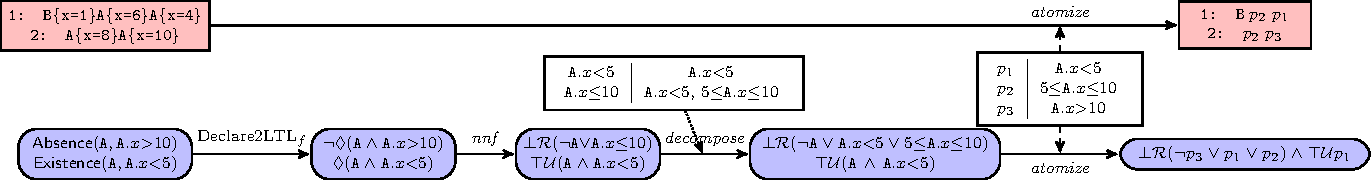
\includegraphics[width=1.3\textwidth]{images/example_1}}
	
	{\hspace{-1.3cm}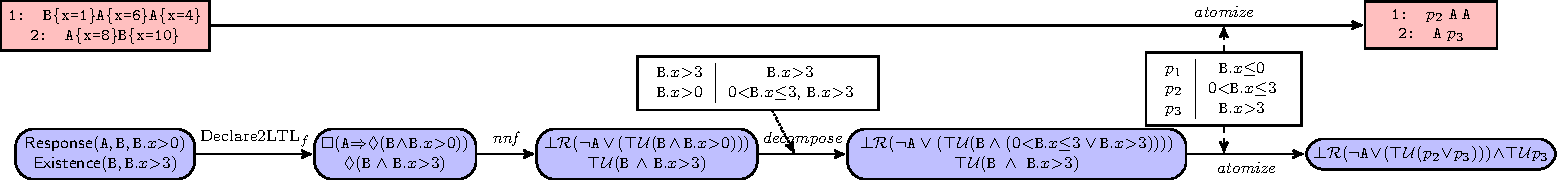
\includegraphics[width=1.3\textwidth]{images/example_2}}
	
	\caption{\texttt{[TODO: Recap]}Two examples (one above, the other below) of input transformation for the $\sigma\tilde{\vDash}\varphi$ Blue boxes represent the Data-Aware Declare model representations, while the red boxes represent the traces' transformation.}\label{fig:twoexamples}
\end{figure}
\begin{lemma}
It always possible to decompose a proposition $\psi(\sigma_i)=\phi_{\texttt{a}}(\sigma_i)\wedge \phi^d(\sigma_i)$ from an LTL$_f$ interpretation of a Declare model $\mathcal{M}$ via a disjunction of atoms in $\Sigma$ such that each event $\sigma_i$ satisfies only one atom in $\Sigma$.
\end{lemma}
\begin{proof}
Figure~\ref{fig:twoexamples} provides an intuitive sketch of the proof. In more detail, after representing each constraint $c_i\in\mathcal{M}$ (step 1) as an LTL$_f$ formula (step 2) in \textit{negated normal form} (\textit{nnf}), we colle
\end{proof}

%Secondly, we can transform the constraint automaton $\mathcal{A}$ into an augmented automaton $\mathcal{A}$ accepting all the traces satisfying $\varphi$
%%
%\begin{proof}	
%Given that non-deterministic finite-state automata (NFA) accept the same language of deterministic finite-state automata \cite{0016921} and that LTL$_f$ formulae can be modeled as DFAs \cite{Westergaard11,Lydia}, there exists a transformation for  $\varphi$ into a deterministic finite-state automaton $\mathcal{A}$ (\textit{constraint automaton}) and one for $\sigma$ into a deterministic finite-state automaton $\mathcal{T}$ (\textit{trace automaton}) as a single (accepting) path such that, if $\mathcal{T}$ is (also) an accepting path for $\mathcal{A}$, then $\sigma\vDash\varphi$ \cite{XuLZ17a}. 
%\end{proof}
%
%
%
%We can show that the declarative conformance checking can be modeled as a trace alignment problem by firstly transforming a Declare model as a deterministic finite-state automaton (DFA) via an LTL$_f$ formula, namely \textit{constraint automaton} $\mathcal{A}$, as well as directly translating the trace $\sigma$ as another DFA, namely \textit{trace automaton} $\mathcal{T}$, which is formed by one single path accepting $\sigma$. Last, we need to show that $\mathcal{A}$ contains the exact path $\mathcal{T}$ 
%
%We can represent $\sigma$ as a DFA $\mathcal{T}=(\Sigma_\sigma,Q_\sigma,q_0^\sigma,\rho_\sigma,F_\sigma)$, namely a \textit{trace automaton} \cite{XuLZ17a}, having having \begin{enumerate*}[label=\emph{\alph*})]
%	\item $\Sigma_\sigma=\Set{\sigma_1,\dots,\sigma_n}$,
%	\item $Q_\sigma=\Set{q_0^\sigma,\dots,q_n^\sigma}$ a set of arbitrary $|\sigma|+1$ states, with
%	\item an initial state $q_0^\sigma$ and
%	\item a set $F=\Set{q_n^\sigma}$ of accepting states, where
%	\item the transition relation $\rho_\sigma(q_i^\sigma,\sigma_i)=q_{i+1}^\sigma$ for each $1\leq i\leq |\sigma|+1$.
%\end{enumerate*}
%Every LTL$_f$ formula can be directly associated to a deterministic finite-state automaton (DFA) $\mathcal{A}=(\Sigma,Q,q_0,\rho,F)$, namely a \textit{constraint automaton}, accepting only the traces satisfying $\varphi$ \cite{Lydia}, having \begin{enumerate*}[label=\emph{\alph*})]
%	\item an input alphabet $\Sigma\subseteq \textsf{Prop}$,
%	\item a finite set $Q$ of states, with
%	\item an initial state $q_0\in Q$ and
%	\item a set $F\subseteq Q$ of accepting states, where
%	\item the latter can be reached from the former via a transition relation $\rho\colon Q\times \Sigma\to Q$.
%\end{enumerate*} Furthermore, 
%
%\[s_{\mathcal{A},\sigma}(q,i)=\begin{cases}
% 	\textbf{true} & i>|\sigma|\wedge q\in F\\
% 	s_{\mathcal{A},\sigma}(q,i+1) & i\leq |\sigma|\wedge \exists! \phi. \rho(q,\phi)
%\end{cases}\]
%
%\bigskip

Secondly, the authors introduced \textit{repair atoms}  \texttt{del\_a} (or \texttt{add\_a}) for each $\texttt{a}\in\Sigma$ respectively remarking that \texttt{a} was removed (or added) in the input trace, while it needs to be added (removed) to make the string accepted. This allows to transform $\mathcal{A}$ into $\mathcal{A}^+$ accepting all the repaired strings $\tilde{t}$ from $t$ \texttt{\color{red}[TODO]}


\texttt{\color{red}[TODO]} we consider insertions and deletions as possible repairs, while substitutions can be modeled by deletions followed by insertions. Synchronizations are \texttt{noops} requiring that a trace $\sigma$ at step $k$ contains a predicate $\phi$. 
\begin{itemize}
	\item synchronization $[\sigma_k\leftrightarrow \phi]$ aborts if $\sigma_k\neq\phi$, for  $1\leq k\leq |\sigma|$
	\item deletion\,\, $[\#\sigma_k\leftarrow \phi]::= \sigma_1\cdots\sigma_{k-1}\sigma_{k}\cdots \sigma_n$,\,\,\, for $n=|\sigma|$, $1\leq k\leq n$, and $\phi=\sigma_k$
	\item insertion $[@\sigma_k\leftarrow \phi]::= \sigma_1\cdots\sigma_{k-1}\phi\sigma_{k}\cdots \sigma_n$, for $n=|\sigma|$ and $1\leq k\leq n$
\end{itemize}
Therefore, any repair  of a trace $\sigma$ can be expressed in terms of a sequence of operations $\texttt{op}_1\cdots \texttt{op}_m$ which, when executed in appearance order, generate a novel trace $\tilde{\sigma}$ from $\sigma$.  \texttt{\color{red}[TODO]}


Last, the amount of repairs can be numerically quantified using a cost function $\mathcal{C}$ returning zero for any synchronization and $1$ otherwise; therefore $cost(\sigma, \tilde{\sigma})$ returns the minimal number of non-synchronization operations\footnote{Formally, $cost(\sigma,\tilde{\sigma})=\min_{\substack{\texttt{op}_1\cdots \texttt{op}_m,\\(\texttt{op}_m\,\circ \cdots\circ\, \texttt{op}_1)(\sigma)=\tilde{\sigma}}}\sum_{1\leq i\leq m}\mathcal{C}(\texttt{op}_m)$} required to obtain $\tilde{\sigma}$ from $\sigma$. Therefore, the conformance checking of a log trace $\sigma$ against a  Declare model represented as an LTL$_f$ formula $\varphi$ as in \cite{XuLZ17a} either returns $\sigma$ with cost zero if $\varphi\vDash\varsigma$ or, otherwise, returns a set of pairs $\Set{\braket{\tilde{\sigma},\texttt{op}_1\cdots\texttt{op}_m}_i}_{1\leq i\leq k, k\in\mathbb{N}}$, where\footnote{Formally, $\sigma\tilde{\vDash}\varphi = \Set{\braket{\tilde{\sigma},\texttt{op}_1\cdots\texttt{op}_m} | cost(\sigma,\tilde{\sigma}) = \min_\mu cost(\sigma,\mu),\;\tilde{\sigma}\vDash\varphi,\; (\texttt{op}_m\,\circ \cdots\circ\, \texttt{op}_1)(\sigma)=\tilde{\sigma}}$.} each trace $\tilde{\sigma}\in S$ is conformant to $\varphi$ and minimizes the alignment cost $cost(\sigma,\tilde{\sigma})$ via a repair sequence $\texttt{op}_1\cdots\texttt{op}_m$. We denote the output of such conformance checking as $\sigma\tilde{\vDash}\varphi$. 



